\documentclass{article}
\usepackage{amsmath}
\usepackage{fancyhdr}
\usepackage{geometry}
\usepackage{amssymb}
\usepackage{graphicx}

% Page margins
\geometry{a4paper, margin=1in}

% Define header
\pagestyle{fancy}
\fancyhf{}
\fancyhead[L]{Student Number: 1462539}
\fancyhead[C]{MAST20005}
\fancyhead[R]{\thepage}

\title{Assignment 1}
\author{}
\date{}

\begin{document}

% Title page
\begin{titlepage}
    \centering
    \vspace*{2in}
    {\Huge \textbf{Assignment 1}}\\[1.5cm]
    {\Large Student Name: Kevin Yu}\\[0.5cm]
    {\Large Student Number: 1462539}\\[0.5cm]
    {\Large Subject Code: MAST20005}\\[0.5cm]
    {\Large Subject Name: Statistics}\\[2in]
    \vfill
    \large \textbf{\today}
    \vfill
\end{titlepage}

\newpage
\section*{Exercise 1}
% Your solution for Exercise 1 goes here.

% Exercise 2
\newpage
\section*{Exercise 2}
% Your solution for Exercise 2 goes here.

\subsection*{Part 1}

$\text{Please note that I have abbreviated } \sum_{i=1}^m \text{ as } \sum \text{ at some places to avoid overcrowding}$

$$
\begin{aligned}
L(\sqrt{ p }) &= \prod_{i=1}^{m} \binom{n}{x_{i}} (\sqrt{ p })^{x_{i}}(1-\sqrt{ p })^{n-x_{i}} \\
&= \prod_{i=1}^m \left[ \binom{n}{x_{i}}\right] (\sqrt{ p })^{\sum x_{i}}(1-\sqrt{ p })^{\sum (n-x_{i})} \\
\implies \ln{L(\sqrt{ p })} &= \ln{\prod_{i=1}^m \left[ \binom{n}{x_{i}}\right]} + \sum_{i=1}^m{(x)}\ln{\sqrt{ p }}+\sum_{i=1}^m{(n-x_{i})}\ln{(1-\sqrt{p})} \\
\implies \frac{d}{d\sqrt{ p }}[\ln{L(\sqrt{ p })})] &= \frac{\sum x_{i} \cdot \frac{1}{2} p^{1/2}}{\sqrt{ p }} + \frac{\left( mn - \sum x_{i} \right) \cdot -\frac{1}{2} p^{1/2}}{1 - \sqrt{ p }} \\
&= \frac{(1-\sqrt{ p })p^{-1/2} \sum x_{i} - mn + \sum x_{i}}{2\sqrt{ p } (1-\sqrt{ p })}
\end{aligned}
$$

$\text{Setting } \frac{d}{d\sqrt{ p }}[\ln{L(\sqrt{ p })})]  = 0 \text{ yields,}$

$$
\begin{aligned}
&(1-\sqrt{ p })p^{-1/2} \sum_{i=1}^m x_{i} - mn + \sum_{i=1}^m x_{i} = 0 \\
\implies &(p^{-1/2} - 1) \sum_{i=1}^m x_{i} - mn + \sum_{i=1}^m x_{i} = 0 \\
\implies &p^{-1/2} \sum_{i=1}^m x_{i} - mn = 0 \\
\implies &p^{-1/2} = \frac{mn}{\sum x_{i}} = \frac{n}{\bar{X}_{m}} \\
\implies &p^{1/2} = \frac{\bar{X}_{m}}{n} \\
& \therefore p = \frac{\bar{X}_{m}^2}{n^2} \qquad \blacksquare
\end{aligned}
$$

\subsection*{Part 2}
% Your solution for Part 2 of Exercise 2 goes here.
$$
\bar{x}_{3} = \frac{1}{3} 
$$

% Exercise 3
\newpage
\section*{Exercise 3}

\subsection*{Part 2}

In addition to the variance, we can calculate
\begin{itemize}
    \item the range (max - min) to measure the spread of the data,
    \item the interquartile range (IQR), the difference between the third and first quartiles, which is less sensitive to outliers,
    \item the median as a measure of central tendency that is less sensitive to outliers.
\end{itemize}

Now, let $y_{(1)}, y_{(2)}, \dots, y_{(9)}$ and $z_{(1)}, z_{(2)}, \dots, z_{(9)}$ be the ordered samples from Sample 1, Sample 2 respectively. \\

For Sample 1, $y_{(1)} = 1.333$ and $y_{(9)} = 1.684$ so the range is $1.684 - 1.333 = 0.351$.  \\ 

For Sample 2, $z_{(1)} = 1.333$ and $z_{(9)} = 1.523$ so the range is $1.523 - 1.333 = 0.190$.  \\

Now to calculate the interquantile range, we recall from the lecture that having $x_{(1)}, x_{(2)}, \dots, x_{(n)}$ as the ordered observations; let the $p$-th quantile of the observations be denoted by $\hat{c}_p$ where $0 < p < 1$. Then, letting $k = 1 + (n-1)p$ and $t$ and $w$ be the whole and fractional part of $k$ respectively, (i.e. $t = \lfloor k \rfloor$ and $w = k - t$),

$$
\hat{c}_p = x_{(t)} + w(x_{(t+1)} - x_{(t)}).
$$
\\
Therefore, for Sample 1, the first quartile ``position'' is at $1 + (9-1)(0.25) = 3$ so the first quartile is $\hat{q}_1 = \hat{c}_{0.25} = y_{(3)} = 1.447$. The third quartile "position" is at $1 + (9-1)(0.75) = 7$ so the third quartile is $y_{(7)} = 1.577$. Hence, the IQR is $1.577 - 1.447 = 0.130$. \\

For Sample 2, the first and third quartile ``position'' is the same as Sample 1. Therefore, the first quartile is $z_{(3)} = 1.333$ and the third quartile is $z_{(7)} = 1.333$. Hence, the IQR is $1.333 - 1.333 = 0$. We also note that since IQR of Sample 2 is 0, so $z_{(9)} = 1.523$ is an extreme outlier. \\

Finally, the median of Sample 1 is $y_{(5)} = 1.529$ and the median of Sample 2 is $z_{(5)} = 1.333$. \\



Ultimately, the range and IQR of Sample 1 are greater than those of Sample 2. This suggests that Sample 1 has a greater variability, while Sample 2 has the same value for the first, second (medium) and third quartiles, indicating that the data is more concentrated around a single value. $\blacksquare$

\begin{figure}[h!]
    \centering
    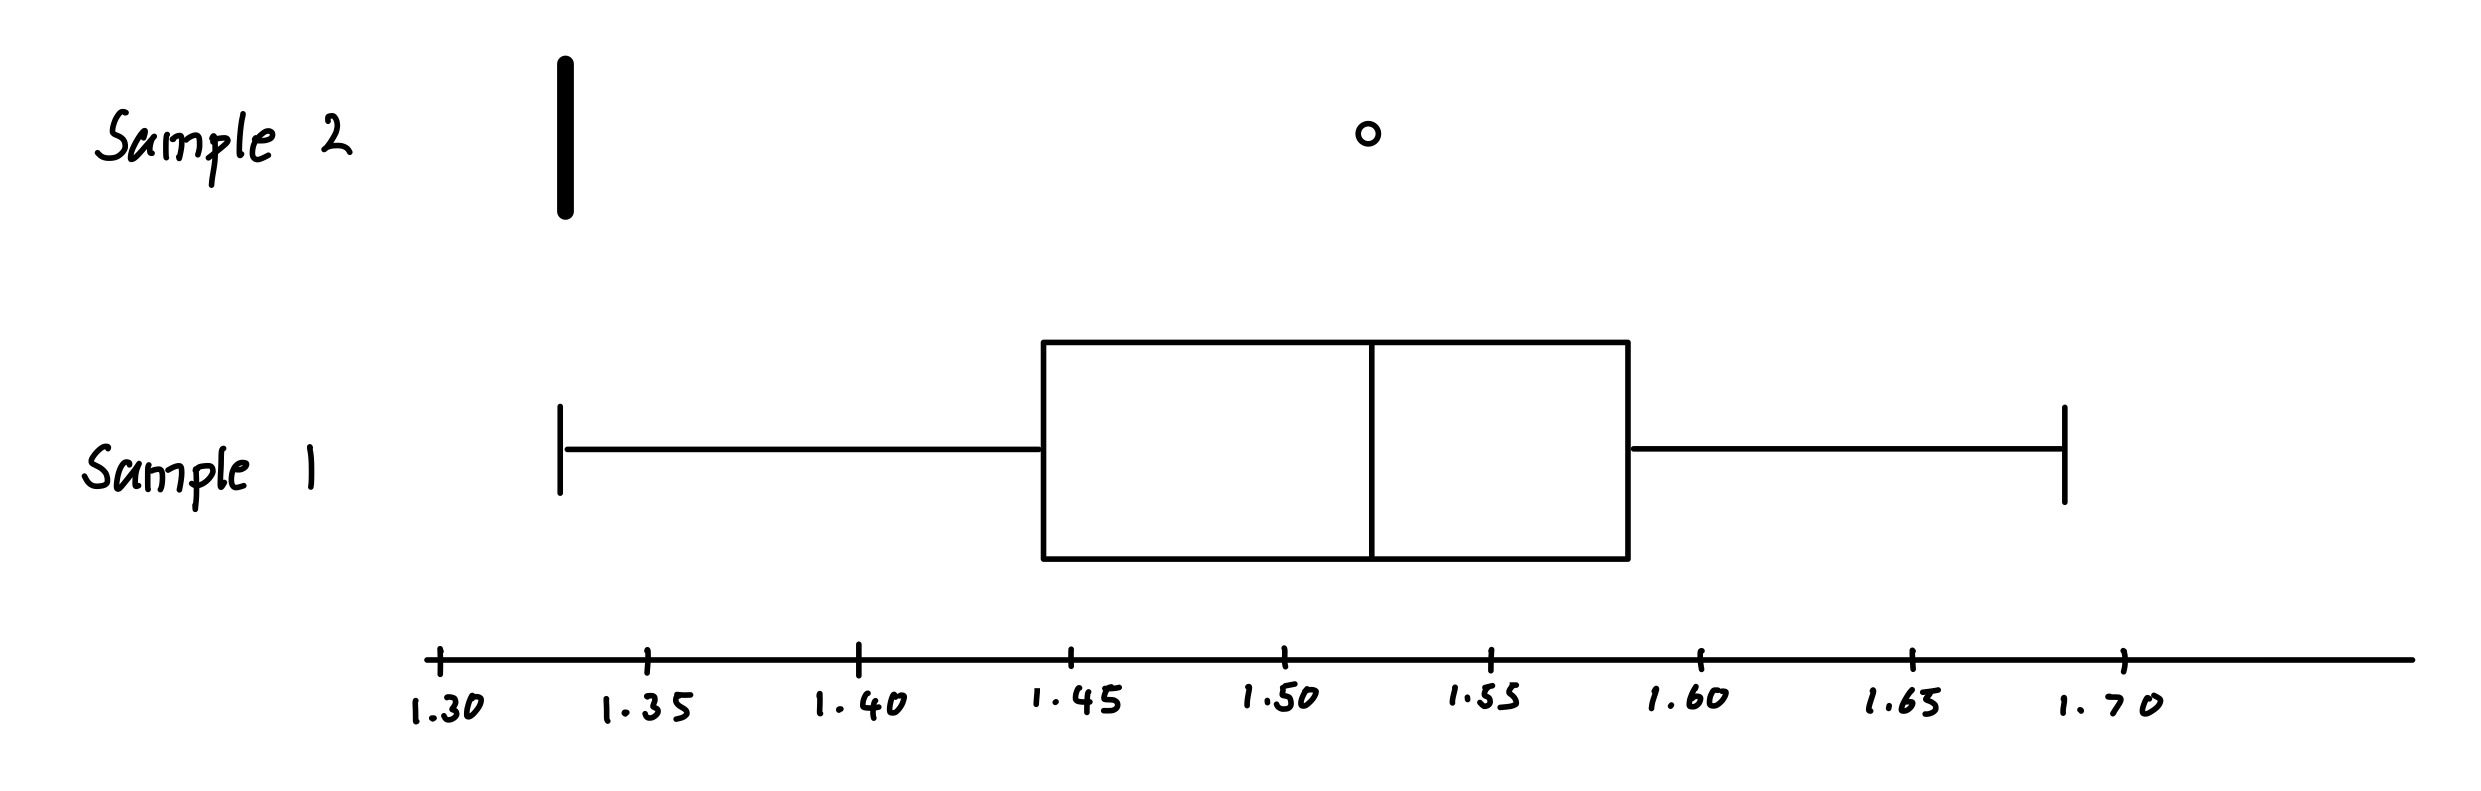
\includegraphics[width=0.8\textwidth]{images/boxplot.jpg}
    \caption{Boxplot of Sample 1 and Sample 2}
    \label{fig:boxplot}
\end{figure}

\newpage
\section*{Exercise 4}

\newpage
\section*{Exercise 5}

\end{document}